\section*{Linear Regression}\; Ass. $Y=X\theta+\epsilon$, $\E[\epsilon]=0$, $\E[\epsilon\epsilon^{\top}]=\sigma^2I_n$
\\
$\cdot\; \E[\epsilon_i^2]\neq0\rightarrow$ weigh. LS $\cdot\; \text{Cov}(\epsilon_i,\epsilon_j)\neq0\rightarrow$ gen. LS $\cdot\; \epsilon\nsim\mathcal{N}\rightarrow$ rob. reg. 
\textbf{LSE}
$\hat \beta = \text{argmin}_\beta ||Y-Xb||_2^2 = (X^\top X)^{-1}X^\top Y$, $\text{Cov}(\hat{\beta})=\sigma^2(X^{\top}X)^{-1}$, $\E[\hat{\beta}]=\beta$,
$\cdot\; \epsilon \sim \mathcal{N}(0,\sigma^2 I)\Rightarrow Y, \hat{\beta}, \hat{Y}, r \sim \mathcal{N}$ and $\hat{\sigma}^2\sim\frac{\sigma^2}{n-p}\chi^2_{n-p}$, where $\hat \sigma^2 = \frac 1 {n-p}RSS$ (unbiased) and $RSS=||Y-X\hat \beta||_2^2=\sum r_i^2$ \\
\textbf{Geometry}: $\hat{Y}=PY$, $r^{\top}x^{(j)}=0\Rightarrow r^{\top}\hat{Y}=0$, $r\in\text{col}(X)^{\perp}$\\
\textbf{Gen LS}: $\Sigma$ known/$\sigma^2G$ w $\sigma$ unknown $\rightarrow$ $\Sigma=CC^{\top}$ (e.g. Cholesky $C\in \nabla-$lower)
$\tilde{Y}=C^{-1}Y=C^{-1}X\beta+C^{-1}\epsilon=\tilde{X}\beta+\tilde{\epsilon}$ $\rightarrow$
$\hat \beta =  (X^{\top} \Sigma^{-1} X)^{-1} X^{\top} \Sigma^{-1} Y$ and $\text{Cov}(\beta)=(X^T\Sigma^{-1}X)^{-1}$\\
$\Sigma=\sigma^2\text{diag}(z_1,\dots,z_n) \rightarrow $ weightLS $\arg\min_{\theta} \sum z_i^{-1} (y_i-x_i^{\top}\theta)^2$
\begin{codebox}{r}{Linear Regression}
fit <- lm(y~x1+x2) # Fit only x1 and x2 (so p=3)
predict(fit, pred.data.frame)
# Manual fit
X <- cbind(1, x1, x2) # p = 3
XtX.inv <- solve(t(X) %*% X)
beta.hat <- XtX.inv %*% t(X.int) %*% y
res <- y - X.int %*% beta.hat # Residuals
RSE <- sqrt(sum(res^2)/(n-p)) #Resid.std.err.=hat(sd)
se.x1 <- RSE * sqrt(XtX.inv[2, 2]) # Std. error of x1
t.val.x1 <- beta.hat[2] / se.x1 # T value of x1
p.val.x1 <- 2*pt(abs(t.val.x1), df=n-p, lower=F)
# Alternative t-value
coef <- summary(fit1)$coefficients
t1 <- coef["x1","Estimate"]/coef["x1","Std. Error"]
# Poly regression
lm(wage~poly(age,4)) # Orthogonal polynomials
lm(wage~poly(age, 4, raw=T)) # Monomial basis
lm(wage~age+I(age^2)+I(age^3)+I(age^4)) # Alternative
summary(y-model\$fitted.values) # Residuals
\end{codebox}

\subsection*{Tests and model selection}
\textbf{Entry-wise test}\\
$H_0: y = X\beta + \epsilon$ with $\beta_j=0$
$H_A: y = X\beta + \epsilon$ with $\beta_j\neq 0$\\
$\frac{\hat \beta_j - \beta_j}{\sqrt{\sigma^2(X^\top X)^{-1}_{jj}}} \sim \mathcal{N}(0,1)$ $\Rightarrow$
t-statistic: $T_j:=\frac{\hat \beta_j}{\sqrt{\hat \sigma^2 (X^\top X)^{-1}_{jj}}} \stackrel{H_0}{\sim} t_{n-p}$\\
\textbf{P-Value}$=P_{H_0}(T>|t|)$, $t=$ obs. instance of $T$.
If $< \alpha$ then reject $H_0$.
\textbf{ANOVA (Analysis of variance)} $\Vert Y-\bar Y \Vert^2=\Vert  \hat Y - \bar Y\Vert^2+\Vert Y-\hat Y\Vert^2$\\
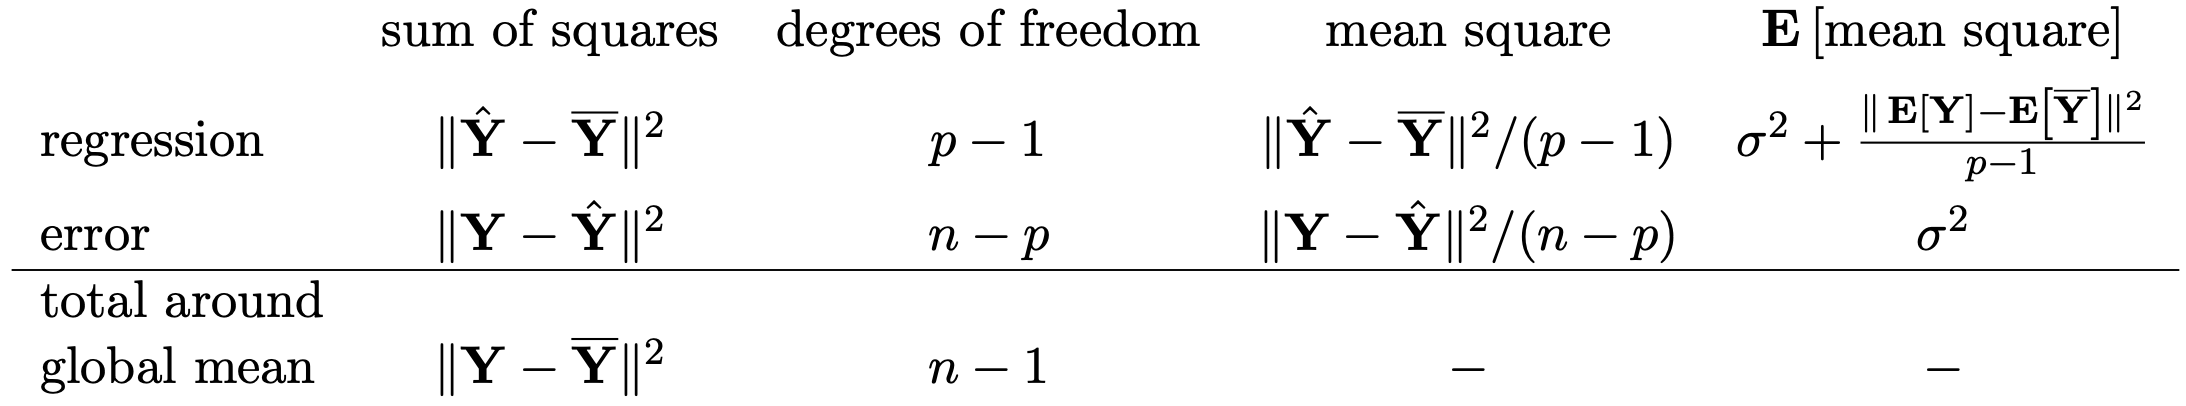
\includegraphics[width = 7cm]{ANOVA.png}
$MSE/\hat{\sigma}^2\rightarrow(H_0:\beta = 0) \Rightarrow F=\frac{\Vert  \hat Y - \bar Y\Vert^2/(p-1)}{\Vert Y- \hat Y\Vert^2/(n-p)}\sim F_{p-1,n-p}$

\begin{codebox}{r}{P-Values \& ANOVA}
fit.smaller <- lm(y ~ x1)
# Anova uses RSS and DoF of largest (last) model, so
# use ascending order!
anova(fit.smaller, fit, fit.all)
# Overall F-Test
fit.empty <- lm(y ~ 1, data=...) # Empty model
anova(fit.empty, fit) # Compare models
# Alternative F-test
Ftest <- summary(fit)$fstatistic
pval <- 1 - pf(Ftest[1], df1=Ftest[2], df2=Ftest[3])
\end{codebox}

BS Alt.: $p=\text{mean}(\#\{\text{m'}:\text{MSE[m'(permuted}[Y],X)] >\text{MSE(m}[Y,X)]\})$

\textbf{R\textsuperscript{2} (Coefficient of determination):} the proportion of the total variation of the response $Y$ around its mean $\bar{Y}$ that is explained by the regression $\hat{Y}$ (via the ANalysis Of VAriance decomposition)
$R^2=\frac{||\hat{Y}-\bar{Y}||^2}{||Y-\bar{Y}||^2}=1-\frac{||Y-\hat{Y}||^2}{||Y-\bar{Y}||^2} = \frac{ESS}{TSS} = 1-\frac{RSS}{TSS}$

\begin{codebox}{r}{R squared}
RSE <- sqrt(sum(residuals(fit)^2)/(n-p))
RSS <- sum(res^2) # Residual sum of squares
TSS <- sum((y - mean(y))^2) # Total sum of squares
R.sq <- 1 - RSS / TSS
AdjR2 <- 1 - (RSS/(n-p))/(TSS/(n-1))
\end{codebox}

\subsection*{Model selection$\;\;$}

BV Tradeoff:
$n^{-1}\sum_{i=1}^n\mathbb{E} \left[ \left( \sum_{j=1}^q \hat{\beta}_j x_{i,j} - m(x_i) \right) ^2 \right]$
$=  n^{-1} \sum_{i=1}^n \left( \mathbb{E}[\sum_{j=1}^q\hat{\beta}_j x_{i, j}] - m(x) \right)^2 + n^{-1}\sum_i \text{Var}(\sum_j \hat{\beta}_j x_{ij})$ and
$n^{-1}\sum_i \text{Var}(\sum_j \hat{\beta}_j x_{ij})=\frac{q}{n} \sigma^2$
\\
Penalized RSS: $||Y - X\beta||^2_2 + \lambda ||\beta||_0$;
\textbf{$\lambda$-choice}: AIC (equiv to $C_p$ for lin Gauss models) $\rightarrow \lambda=2\hat{\sigma}^2$; BIC $\rightarrow \lambda=\log(n)\hat{\sigma}^2$; $\lambda$ by CV
\\
\textbf{Forward Selection:} 1) Fit $M_0$ 2) For $k=0,...,p-1$ fit all $p-k$ models with 1 additional predictor and select best (smallest RSS): $M_k$. 3) Select best among $M_0,....,M_p$ using CV or penalized RSS. \\
\textbf{Backward Selection:} 1) Fit $M_p$ (full model). 2) For $k=p,p-1,...,1$: fit all $k$ models that drop one perdictor in $M_k$. Choose best (smallest RSS): $M_{k-1}$. 3) Select best among $M_0,...,M_p$ using CV or penalized RSS.
\begin{codebox}{r}{Stepwise methods}
library(leaps)
# Try all the submodels
regfit.full=regsubsets(Salary~., data=..., nvmax=19)
# Forward stepwise (method="backward" for backward)
regfit.full=regsubsets(Salary~., data=..., nvmax=19, method="forward")
\end{codebox}

\subsection*{R Diagnostic plots} \#1 Tukey-Anscombe Checks $E(\epsilon)=0$.
linear trend, do: $Y\mapsto\log Y$; sqrt trend, do: $Y\mapsto\sqrt{Y}$; sq trend: add $x^2$; groups: add categs; else weightLR
\#2 Q-Q Plot not linear: then $r,\epsilon\nsim\mathcal{N}$ (still all fine). \#3 Scale-Location: should be flat, else $\text{Var}(\epsilon_i)=\sigma^2$ violated (p-values wrong). \#4/\#5 Cook distance: shows if some data points have a larger impact on the fit than others (outliers). Note: can't detect if the residuals are correlated with these plots!

\textbf{Categorical Variables:} 
For two levels:$y_i = \beta_1 x_{i1}+...+\beta_p x_{ip} + \lambda d_{is} + \epsilon_i$ 
so if $i$ is in category, then $d_{is}=1$ else $d_{is}=0$. This acts as a different intercept ($E(y_i)-E(y_j)=\lambda$). If more categories, add more dummy variables.

\begin{codebox}{r}{Categ. var. by hand \& LOOCV}
a1 <- (levels(shelveloc)[2]==shelveloc)*1
lcv<-mean((residuals(fit)/(1-lm.influence(fit)$h))^2)
# Creating Categorical Variables
Carseats$High=ifelse(Carseats$Sales<=8,"No","Yes")
\end{codebox}


%\textbf{Interaction:} dummy can also influence slope: add term $\delta d_i x_i$, can influence interaction between predictors: add term $\delta x_{i2} x_{i3}$, can influence other categorical variable: add term $\delta d_{i1}d_{i2}$.

